\documentclass[11pt,a4paper]{article}

\usepackage[margin=2.5cm]{geometry}
\usepackage[T1]{fontenc}
\usepackage[utf8]{inputenc}
\usepackage{times}
\usepackage{setspace}
\usepackage{hyperref}
\usepackage{booktabs}
\usepackage{listings}
\usepackage{enumitem}
\usepackage{amsmath}
\usepackage{graphicx}

\hypersetup{colorlinks=true,linkcolor=black,citecolor=black,urlcolor=blue}
\lstset{
  basicstyle=\ttfamily\scriptsize,
  breaklines=true,
  frame=single,
  columns=fullflexible,
  keepspaces=true,
  showstringspaces=false
}
\onehalfspacing
\setlength{\parskip}{0.35em}
\setlength{\parindent}{1.2em}
\setcounter{tocdepth}{2}
\raggedbottom

\title{\textbf{GeoLineage: A Provenance-First GeoETL Pipeline for\\
Reproducible Geospatial Data Supply Chains}}
\author{Suad Arzimanli\\
\texttt{suad.arzimanli@gmail.com}}
\date{}

\begin{document}
\maketitle

\begin{abstract}
Cloud-hosted, frequently updated sources such as STAC catalogs are now common in geospatial and Earth-observation (EO) pipelines. A recurring issue is missing provenance: it is rarely clear which inputs and parameters produced a given output, or how the input set changed from one run to the next. That gap undercuts reproducibility, auditability, and the chance to skip redundant work when re-running pipelines---a problem already highlighted for geodata web services~\cite{cannata2025} and for GIScience in general~\cite{nuest2018,nuest2020}.

This paper describes~\textbf{GeoLineage}, a provenance-first GeoETL pipeline that (1)~ingests spatiotemporal assets from a STAC catalog via bbox and collection query, (2)~writes an analysis-ready footprint product (GeoParquet in the reference implementation; GeoJSON in a thin hosted demo), (3)~emits a machine-readable lineage record every run, (4)~supports a ``diff since last run'' (added, removed, unchanged inputs), and (5)~reuses the previous run's output when the input set is unchanged (\emph{minimum recompute}). The pipeline is catalog-agnostic and has been tried on two STAC-based sources (Element84 Earth Search and Copernicus Data Space Ecosystem). Correctness is checked through parameter-variation experiments and an automated suite for lineage completeness, diff behaviour, and reuse. In repeated runs the suite reported 4/4 PASS; identical-parameter reruns produced no extra output files and still wrote a new lineage record each time. A stress test with 20 consecutive identical runs gave a 100\% reuse rate and 0\% spurious diff under the conditions used. The results are consistent with lineage artifacts being enough for this pipeline to answer ``what produced this output?'' without an external service, with the input-set diff correct under parameter change, and with minimum recompute avoiding duplicate outputs while keeping a full audit trail. A companion hosted demonstration preserves the same receipt contract with a GeoJSON footprint product and downloadable receipts, indicating the pattern is format-agnostic at the product layer.

\noindent\textbf{Keywords:} provenance; lineage; reproducibility; geospatial ETL; STAC; GeoParquet; minimum recompute.
\end{abstract}

{\small\tableofcontents}
\clearpage

\section{Introduction}

\subsection{Motivation and Problem}
Supply chains for geospatial data are moving away from static, file-based workflows toward cloud-native ones: STAC APIs~\cite{stac} for discovery, formats like COG and GeoParquet~\cite{geoparquet} for analysis-ready data, and frequent updates to basemaps and EO products. Pipelines are re-run on a schedule or on demand. Outputs can change over time not just when code or parameters change, but when upstream catalogs or datasets change. Two questions then matter, and in practice they are often hard to answer:

\begin{itemize}[leftmargin=1.4em]
  \item \textbf{What produced this output?} Which catalog, which search parameters (e.g.\ bbox, collection, datetime, limit), and which concrete input assets (item identifiers, hrefs) were used? What transform was applied and with what parameters?
  \item \textbf{What changed between this run and the last?} Which input assets were added, removed, or unchanged? This is essential for understanding why results differ and for deciding what needs to be recomputed.
\end{itemize}

Cannata et al.~\cite{cannata2025} spell out the reproducibility issue for work that depends on geodata web services: even when services aim for FAIR, you often cannot get back the \emph{same} dataset later---persistent IDs and version pinning are missing, and updates break replicability. N\"ust et al.~\cite{nuest2018} looked at reproducibility in GIScience via AGILE conference papers and found a broad gap; later work~\cite{nuest2020} describes reproducibility reviews and guidelines.

\subsection{Research Questions and Contributions}
This paper addresses three research questions:

\begin{itemize}[leftmargin=1.4em]
  \item \textbf{RQ1.} Can a compact, machine-readable lineage record answer ``what produced this output?'' for a STAC$\rightarrow$footprint pipeline without an external lineage service?
  \item \textbf{RQ2.} Can an input-set diff (added / removed / unchanged) correctly reflect parameter change between consecutive runs?
  \item \textbf{RQ3.} Can minimum recompute avoid rewriting identical footprint products while still emitting a new lineage record (audit trail)?
\end{itemize}

\noindent\textbf{Contributions.}
\begin{enumerate}[leftmargin=1.4em]
  \item A \textbf{catalog-agnostic} provenance-first GeoETL reference: STAC ingest, footprint product, lineage JSON, diff, and minimum recompute in one open pipeline.
  \item A minimal \textbf{lineage schema} that records query parameters, concrete input assets, transform steps, and checksummed outputs, sufficient to answer RQ1 for this pipeline.
  \item An operational definition of \textbf{input-set identity} and experiments showing correct diff (RQ2) and reuse (RQ3) under controlled parameter change.
  \item An automated \textbf{validation suite} and stress test quantifying reuse rate and spurious diffs under repeated identical queries.
  \item A \textbf{contract-preserving hosted demonstration} of the same receipt schema with a GeoJSON footprint product, downloadable receipts, first-run null-diff semantics, and minimum recompute---showing the provenance pattern is not tied to a single on-disk format.
\end{enumerate}

\subsection{Scope}
We study retrospective, dataset-level lineage for a single-transform footprint product. We do not claim a full W3C PROV store, ISO~19115 XML packaging, or an OpenLineage event backend; related work positions those dialects, and offline mapping labs document possible adapters. Catalog version pinning is out of scope: we record what the catalog returned at query time.

\section{Related Work}

\subsection{Reproducibility and Geodata Web Services}
Cannata et al.~\cite{cannata2025} argue that geodata web services undermine classic ``rerun the notebook'' reproducibility because upstream content drifts. N\"ust et al.~\cite{nuest2018,nuest2020} frame GIScience reproducibility culture and review practice. Howe and Tullis~\cite{howe2022} discuss context needed for geospatial UAS reproducibility. GeoLineage does not pin STAC catalogs; instead it records \emph{what was returned at query time}.

\subsection{Provenance and Lineage in Geospatial Workflows}
W3C PROV~\cite{prov} provides Entity / Activity / Agent relations. ISO~19115 lineage~\cite{iso19115} models sources and process steps. Closa et al.~\cite{closa2019,closa2021} integrate ISO geospatial lineage with OGC WPS and study provenance-based queries. Yue et al.~\cite{yue2010} track metadata through geospatial service chaining. Zhang et al.~\cite{zhang2020} couple OGC WPS with W3C PROV. Di et al.~\cite{di2013} implement ISO~19115/-2 lineage in web workflows. Semantic approaches to GIService provenance continue this line~\cite{ijgi2023}. OpenLineage~\cite{openlineage} offers job/run/dataset event streams for modern platforms. Fine-grain PROV (feature/attribute) appears in the Mas\'o/Closa line~\cite{masoclos2017}.

GeoLineage emits a \textbf{retrospective JSON receipt} per run. That is closer to a file-side research-object fragment than to a live OpenLineage emitter or a PROV triple store. The schema can be mapped to those dialects; the reference implementation keeps the receipt self-contained so RQ1 can be answered locally.

\subsection{Versioning, FAIR, and Minimum Metadata}
Gonz\'alez--Cebri\'an et al.~\cite{gonzalez2024} and Thompson et al.~\cite{thompson2023} discuss FAIR dataset versioning and map dissemination. Content-addressed reuse (checksum equality) is a practical minimum for ``same bytes.'' GeoLineage uses input-set identity plus output checksum for reuse and records \texttt{reused\_from\_run\_id} when product bytes are not rewritten---an approximation of versioning, not a minted DOI or STAC Version identifier.

\subsection{STAC and Analysis-Ready Formats}
STAC~\cite{stac} standardises discovery. The Processing extension~\cite{stacproc} can attach process metadata to Items. GeoParquet~\cite{geoparquet} is a strong on-disk ARD choice for tabular footprints. The reference GeoLineage implementation writes footprint GeoParquet; a companion hosted demo uses GeoJSON for the same logical product (checksummed footprints) without changing the lineage contract.

\section{Method}
\label{sec:method}

\subsection{Pipeline Overview}
The pipeline is linear and consists of four logical phases: \textbf{Ingest}, \textbf{Transform}, \textbf{Lineage}, and \textbf{Diff}. Optionally, \textbf{Minimum recompute} is applied before the transform phase.

Figures~\ref{fig:app-run}--\ref{fig:app-history} show the same contract in the hosted browser UI. User parameters (\texttt{bbox}, \texttt{catalog\_url}, \texttt{collection}, \texttt{max\_items}, optional \texttt{datetime}) drive a STAC ingest; the result is a list of Items (id, href, geometry). A minimum-recompute check compares the current run's input set to the latest run's input set; if equal, the pipeline reuses the latest run's output and sets \texttt{reused\_from\_run\_id}. Otherwise, the transform produces a footprint product and computes its SHA-256. A lineage record is written for every run. Finally, a diff against the previous run reports added, removed, and unchanged inputs.

\subsection{Ingest}
\begin{itemize}[leftmargin=1.4em]
  \item \textbf{Input:} \texttt{catalog\_url}, \texttt{collection}, \texttt{bbox} (minx, miny, maxx, maxy in WGS84), \texttt{max\_items}, and optionally \texttt{datetime} (temporal filter).
  \item \textbf{Process:} Open the STAC catalog (e.g.\ with \texttt{pystac-client}), search, and retrieve Items. From each item extract \texttt{id}, \texttt{href}, and optionally a checksum from asset metadata if provided. Prefer the Item self link for \texttt{href}; if absent, fall back to the first asset href (implementation choice; see href semantics in Section~\ref{sec:limitations}).
  \item \textbf{Output:} A list of \texttt{InputAsset} records and Item objects for transform; \texttt{search\_params} stored for lineage.
\end{itemize}

\subsection{Minimum Recompute}
\paragraph{Definition 1 (Input Identity Key).}
For an asset, $k(\mathrm{asset})=(\mathrm{id},\mathrm{checksum})$ if checksum is present, else $(\mathrm{id})$. Input-set equality and reuse logic use this key throughout.

\paragraph{Definitions (input-set equality).}
\begin{itemize}[leftmargin=1.4em]
  \item \textbf{Input-set key:} as in Definition~1.
  \item \textbf{Equality:} the current run's input set equals the latest run's if and only if the sets of keys are equal (order-independent).
  \item \textbf{Determinism requirement:} for reuse to be correct, the transform must be deterministic given the input items (geometry and datetime extraction) and fixed parameters (CRS, schema).
\end{itemize}

\paragraph{Process.}
Load the latest run's lineage. Compare current \texttt{input\_assets} to the latest using key equality. If equal, set \texttt{output\_assets} to the latest run's and set \texttt{reused\_from\_run\_id}; do not call the transform. If not equal, proceed to transform. In both cases a \emph{new} lineage record is written (new \texttt{run\_id}, current timestamp), so history remains complete.

\subsection{Transform}
For each item, extract geometry (footprint), item id, and datetime. Build a GeoDataFrame with columns \texttt{id}, \texttt{datetime}, \texttt{geometry} in EPSG:4326. Write GeoParquet and compute SHA-256 of the written file. These form one entry in \texttt{output\_assets}.

\subsection{Lineage Record}
Each run produces a JSON document with: \texttt{run\_id} (UUID), \texttt{timestamp} (ISO~8601 UTC), \texttt{catalog\_url}, \texttt{search\_params}, \texttt{input\_assets}, \texttt{transform\_steps}, and \texttt{output\_assets}. Storage is one file per run under \texttt{lineage\_runs/runs/<run\_id>.json}, so ``what produced this output?'' can be answered by loading the lineage for a given \texttt{run\_id}.

The implementation also emits a \textbf{lineage DAG} (nodes: \texttt{input\_set}, \texttt{output\_asset}; edges: transform name and parameters) stored in the same JSON, so a helper can traverse backward from any output to the transform and input set(s). A CLI helper (\texttt{scripts/query\_lineage.py}) answers ``what produced this output?'' by \texttt{run\_id} or output path; the hosted UI surfaces the receipt (including \texttt{lineage\_dag}) on the run-detail page. The DAG design is compatible with STACD-style lineage and queryable geospatial provenance as discussed in related models~\cite{closa2019,closa2021,zhang2020}.

\subsection{Diff}
\begin{itemize}[leftmargin=1.4em]
  \item \textbf{Input:} The current run's lineage (in memory) and the lineage store.
  \item \textbf{Process:} Determine the previous run (next-oldest timestamp). Compare \texttt{input\_assets} using Definition~1. Classify each asset as \textbf{Added} (in current, not previous), \textbf{Removed} (in previous, not current), or \textbf{Unchanged} (in both).
  \item \textbf{Output:} Counts and lists of added, removed, and unchanged assets (CLI and hosted UI; Figure~\ref{fig:app-diff}). If no previous run exists, diff is omitted (first-run semantics); this avoids inventing a spurious baseline.
\end{itemize}

\section{Design and Implementation}

\subsection{Lineage Schema (JSON)}
Required fields: \texttt{run\_id}, \texttt{timestamp}, \texttt{catalog\_url}, \texttt{search\_params}, \texttt{input\_assets}, \texttt{transform\_steps}, \texttt{output\_assets}. Recommended extensions for stronger reproducibility claims include \texttt{pipeline\_version}, \texttt{environment}, \texttt{execution}, \texttt{reuse}, and signatures such as
\[
\texttt{query\_signature}=\mathrm{SHA256}(\texttt{catalog\_url}\Vert\texttt{bbox}\Vert\texttt{collection}\Vert\texttt{max\_items}\Vert\texttt{datetime}),
\]
and an \texttt{input\_signature} over sorted Definition~1 keys. These signatures make reuse and diff checks more principled and support a reproducibility score. Transform step elements may optionally include \texttt{step\_id} and \texttt{produces} (paths) for future multi-step DAG compatibility. The current implementation emits the required set; the paper proposes the recommended fields for stronger claims. The schema is minimal and self-contained; it can be extended or mapped to PROV or STAC Processing metadata~\cite{prov,stacproc}.

\subsection{File Layout and Data Sources}
\begin{itemize}[leftmargin=1.4em]
  \item \textbf{Outputs:} \texttt{outputs/<run\_id>/footprints.parquet} (unless reused; then the path points to the previous run's directory).
  \item \textbf{Lineage:} \texttt{lineage\_runs/runs/<run\_id>.json}.
  \item \textbf{Configurability:} optional \texttt{output\_dir} and \texttt{lineage\_dir} (e.g.\ \texttt{validation\_outputs}, \texttt{validation\_lineage\_runs}).
\end{itemize}
The pipeline is \textbf{catalog-agnostic}. Two sources were integrated and tested: (1)~Element84 Earth Search~\cite{earthsearch} (e.g.\ \texttt{sentinel-2-c1-l2a}), and (2)~Copernicus Data Space Ecosystem STAC~\cite{copernicus}.

\subsection{Implementation}
Python~3.10+: \texttt{pystac-client}, GeoPandas, PyArrow, and the standard library for JSON, SHA-256, and UUID. CLI: \texttt{python -m scripts.run\_pipeline} with \texttt{--bbox}, \texttt{--catalog}, \texttt{--collection}, \texttt{--max-items}, \texttt{--out-dir}, \texttt{--lineage-dir}. An optional local Streamlit demo remains available for offline exploration; evaluation claims in Section~\ref{sec:eval} are grounded in the open reference pipeline and its validation scripts.

\paragraph{Companion hosted demonstration.}
A browser UI exercises the \emph{same} lineage contract with a footprint product serialised as GeoJSON (\texttt{application/geo+json}) instead of GeoParquet. Figures~\ref{fig:app-run}--\ref{fig:app-history} show the live screens: search parameters and bbox (Figure~\ref{fig:app-run}); run detail with footprint map and scene diff (Figures~\ref{fig:app-detail}--\ref{fig:app-diff}); downloadable JSON receipt including \texttt{lineage\_dag} (Figure~\ref{fig:app-receipt}); and history with \texttt{complete}/\texttt{reused} status (Figure~\ref{fig:app-history}). Each completed run emits a downloadable lineage receipt (required fields plus \texttt{reused\_from\_run\_id} when applicable), a checksummed footprint download, and an added/removed/unchanged diff---omitted on the first run when no prior receipt exists. Minimum recompute compares input-id sets across receipts exactly as in Definition~1 (id-only when checksums are absent). The hosted UI shows that RQ1--RQ3 transfer to a browser-facing footprint product without changing the receipt schema.

\begin{figure}[ht]
\centering
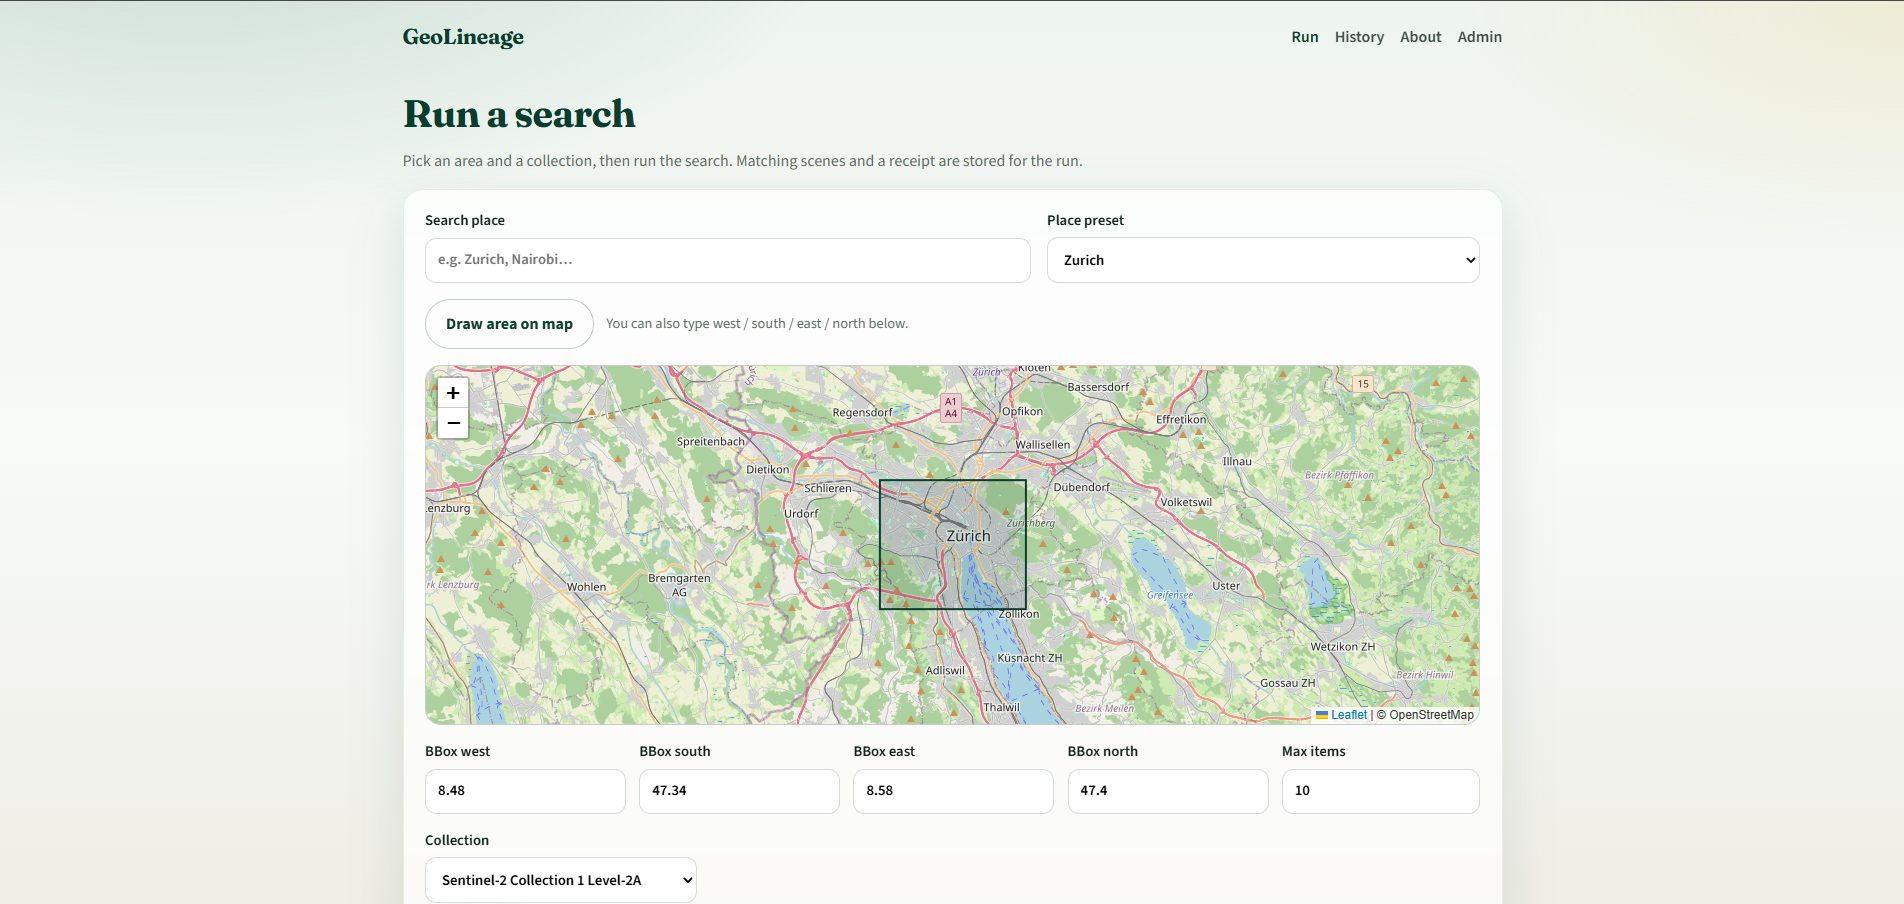
\includegraphics[width=\textwidth]{figures/app_run.png}
\caption{Hosted UI: run form with place/bbox controls, map draw box, \texttt{max\_items}, and STAC collection.}
\label{fig:app-run}
\end{figure}

\begin{figure}[ht]
\centering
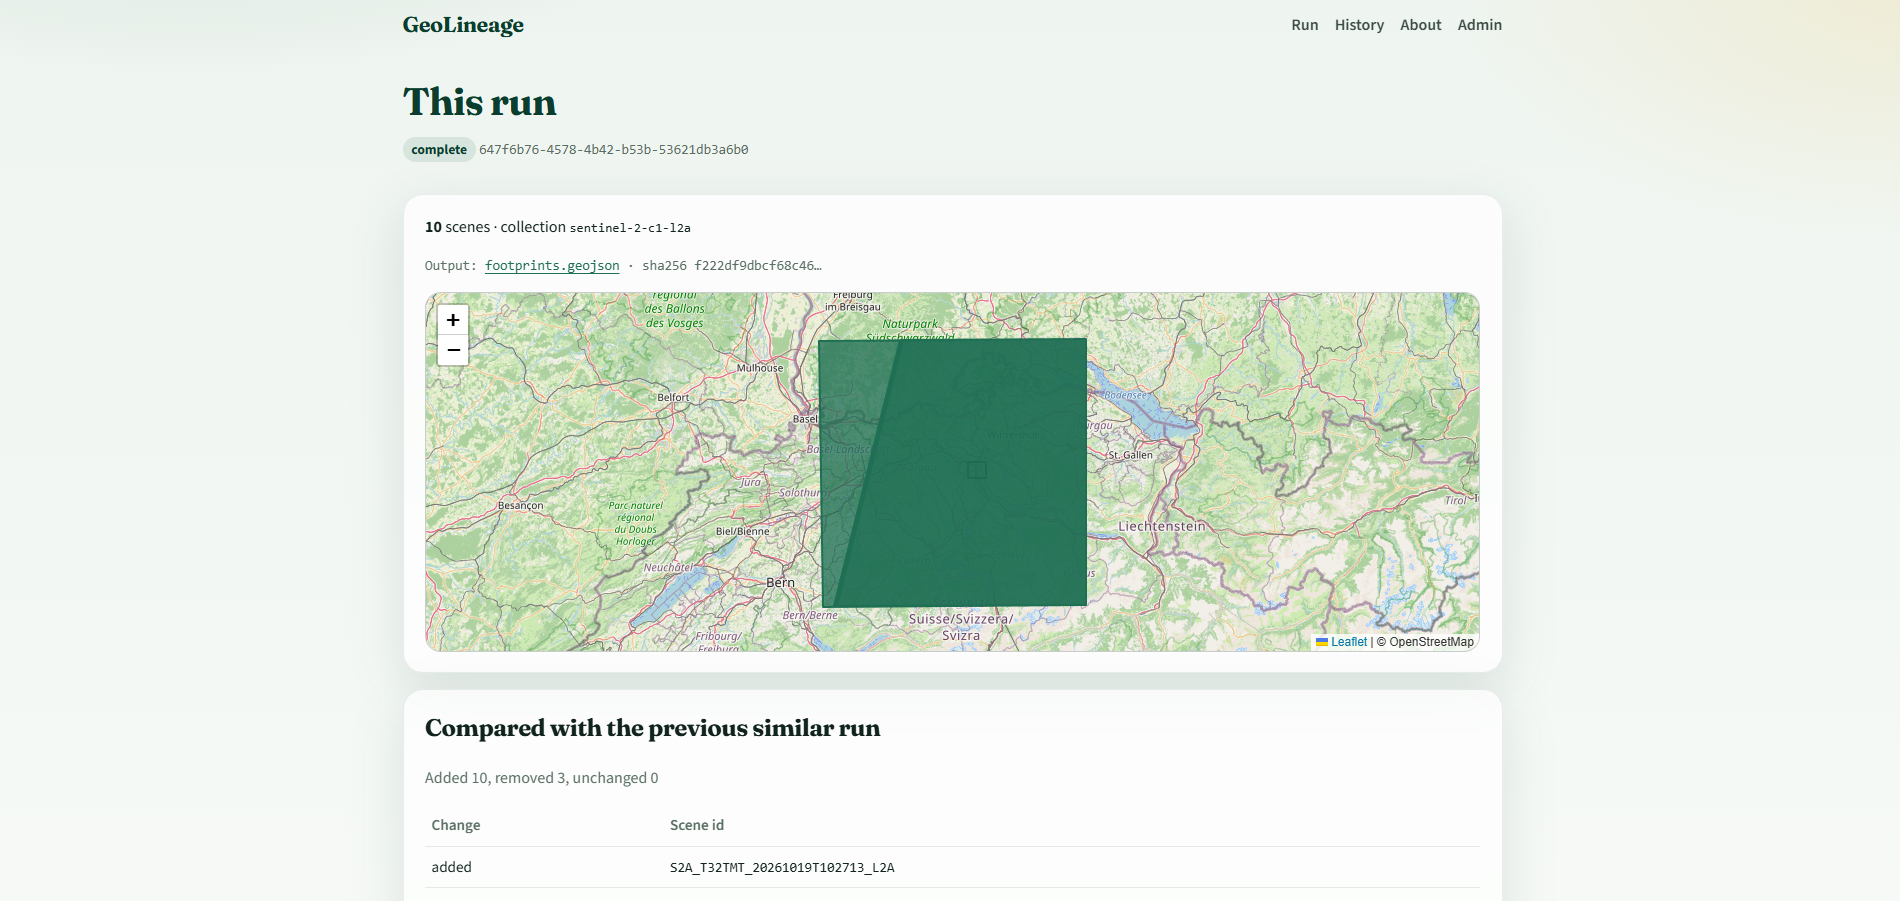
\includegraphics[width=\textwidth]{figures/app_run_detail.png}
\caption{Hosted UI: run detail with footprint map, output GeoJSON path/checksum, and start of the scene diff.}
\label{fig:app-detail}
\end{figure}

\begin{figure}[ht]
\centering
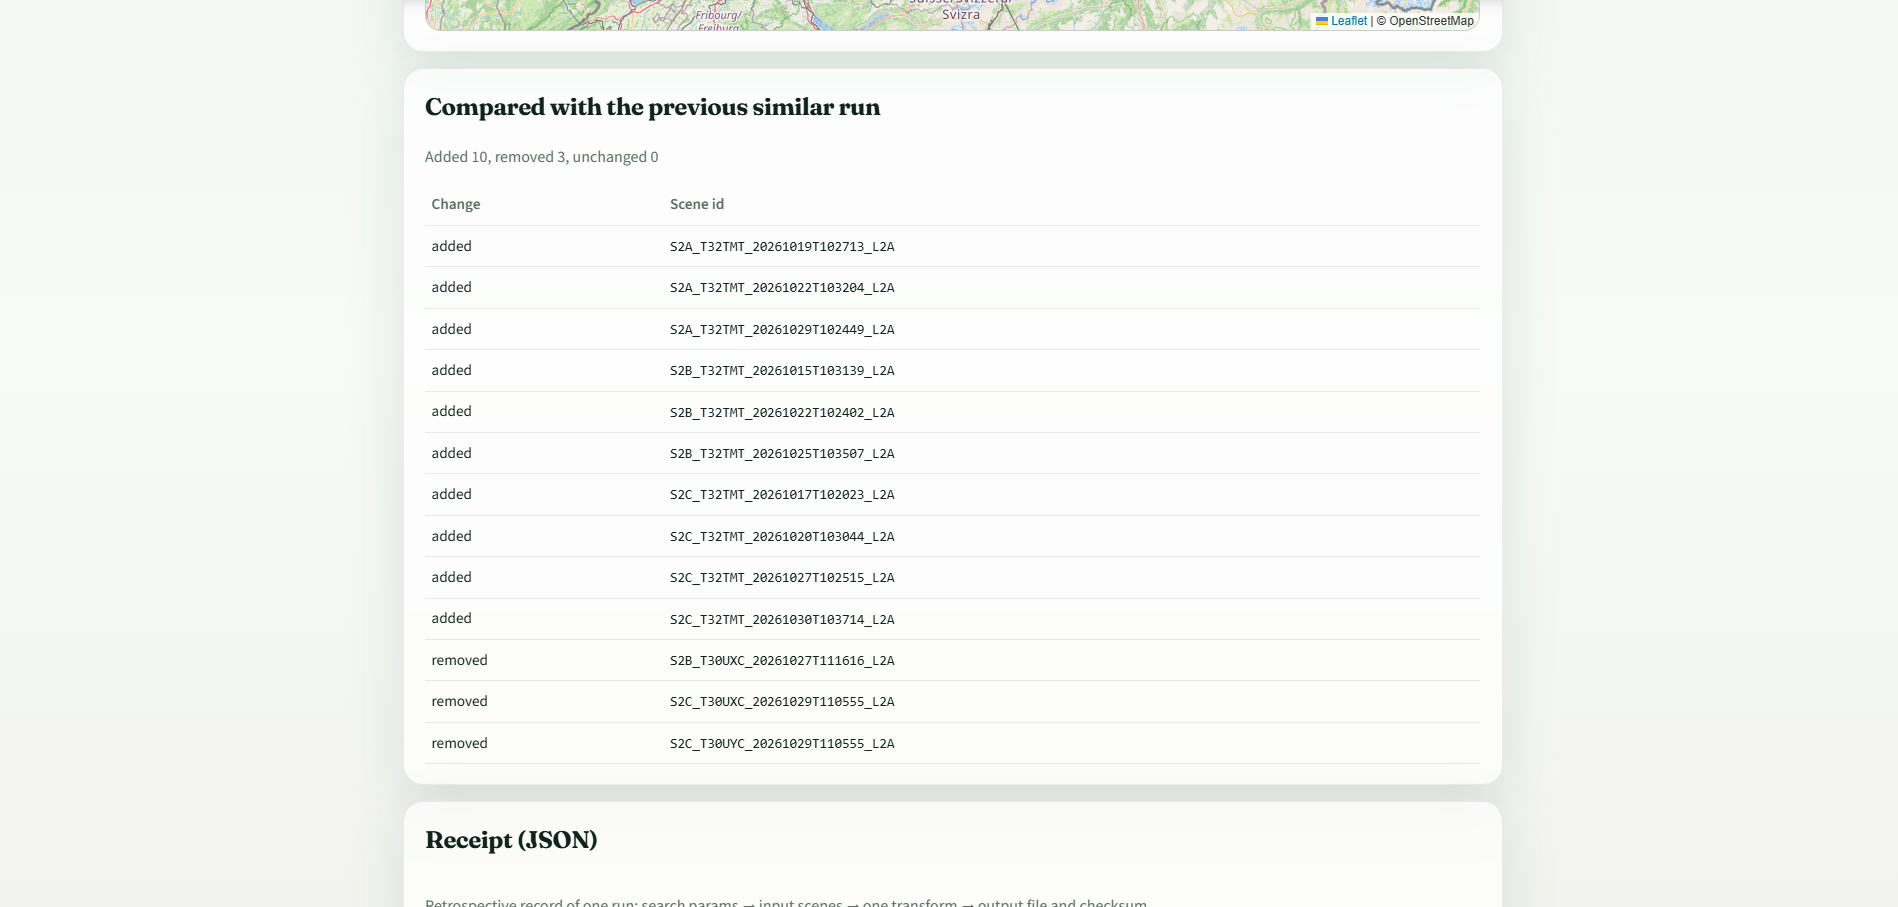
\includegraphics[width=\textwidth]{figures/app_diff.png}
\caption{Hosted UI: input-set diff vs the previous similar run (added / removed scene ids) and the receipt section below.}
\label{fig:app-diff}
\end{figure}

\begin{figure}[ht]
\centering
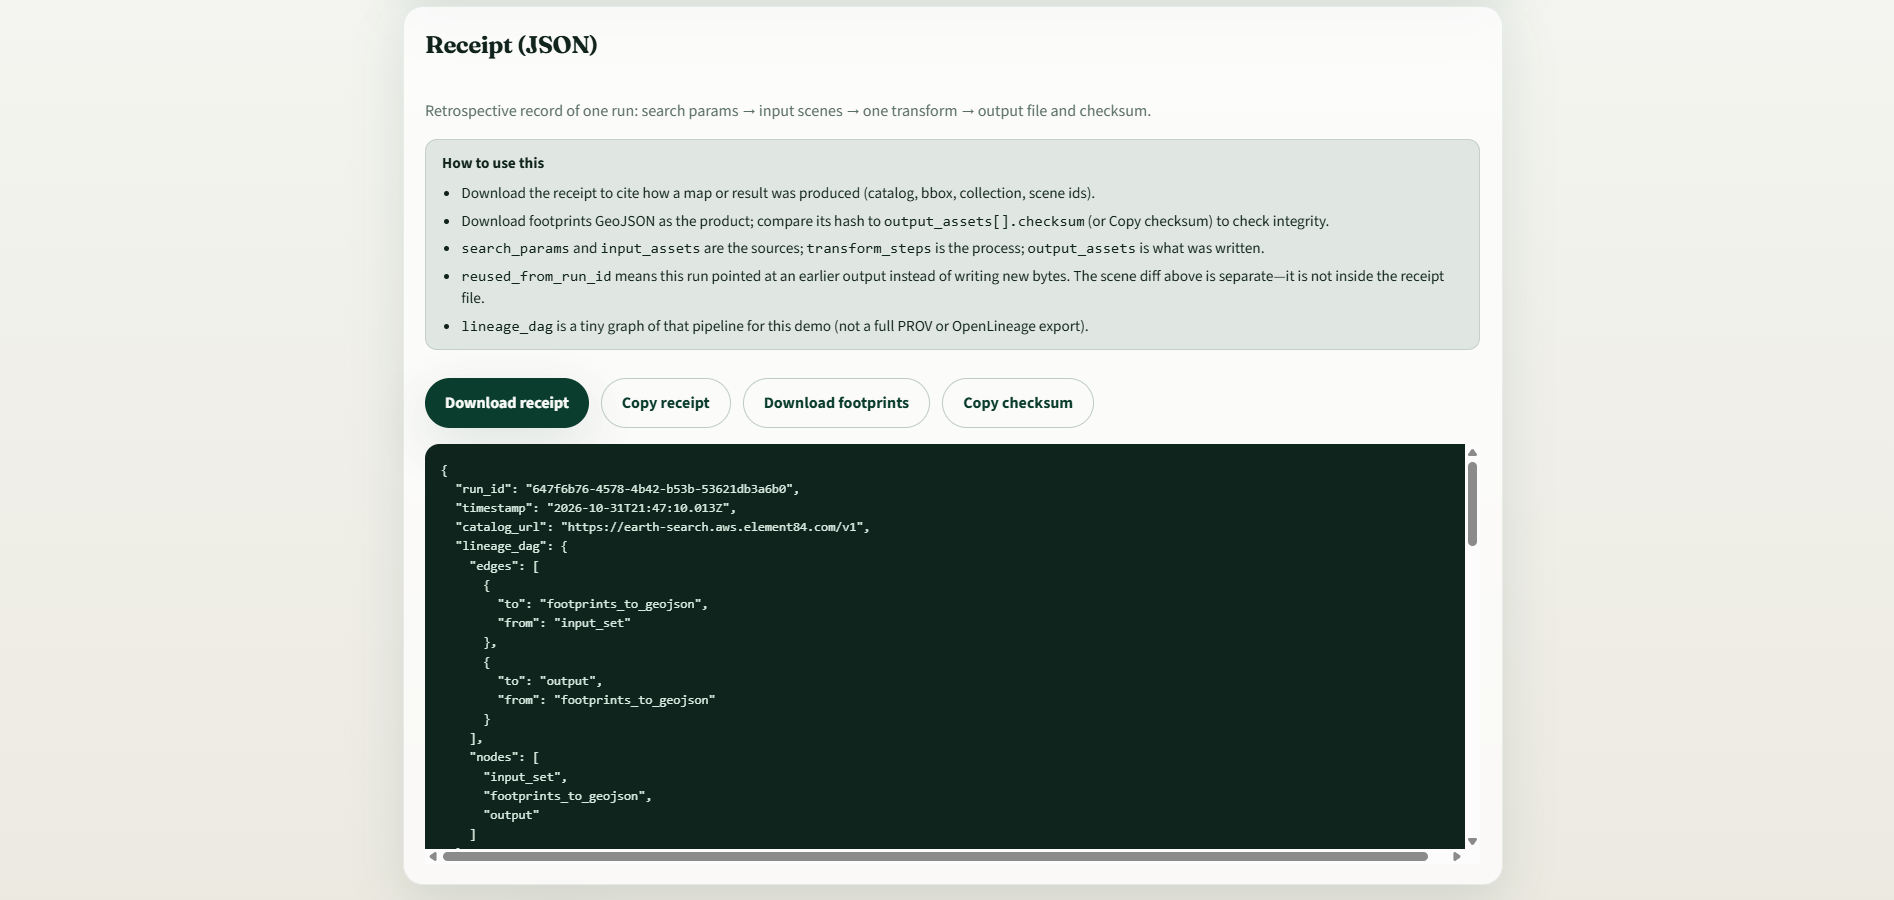
\includegraphics[width=\textwidth]{figures/app_receipt.png}
\caption{Hosted UI: downloadable lineage receipt (JSON) with guide text, checksum actions, and \texttt{lineage\_dag}.}
\label{fig:app-receipt}
\end{figure}

\begin{figure}[ht]
\centering
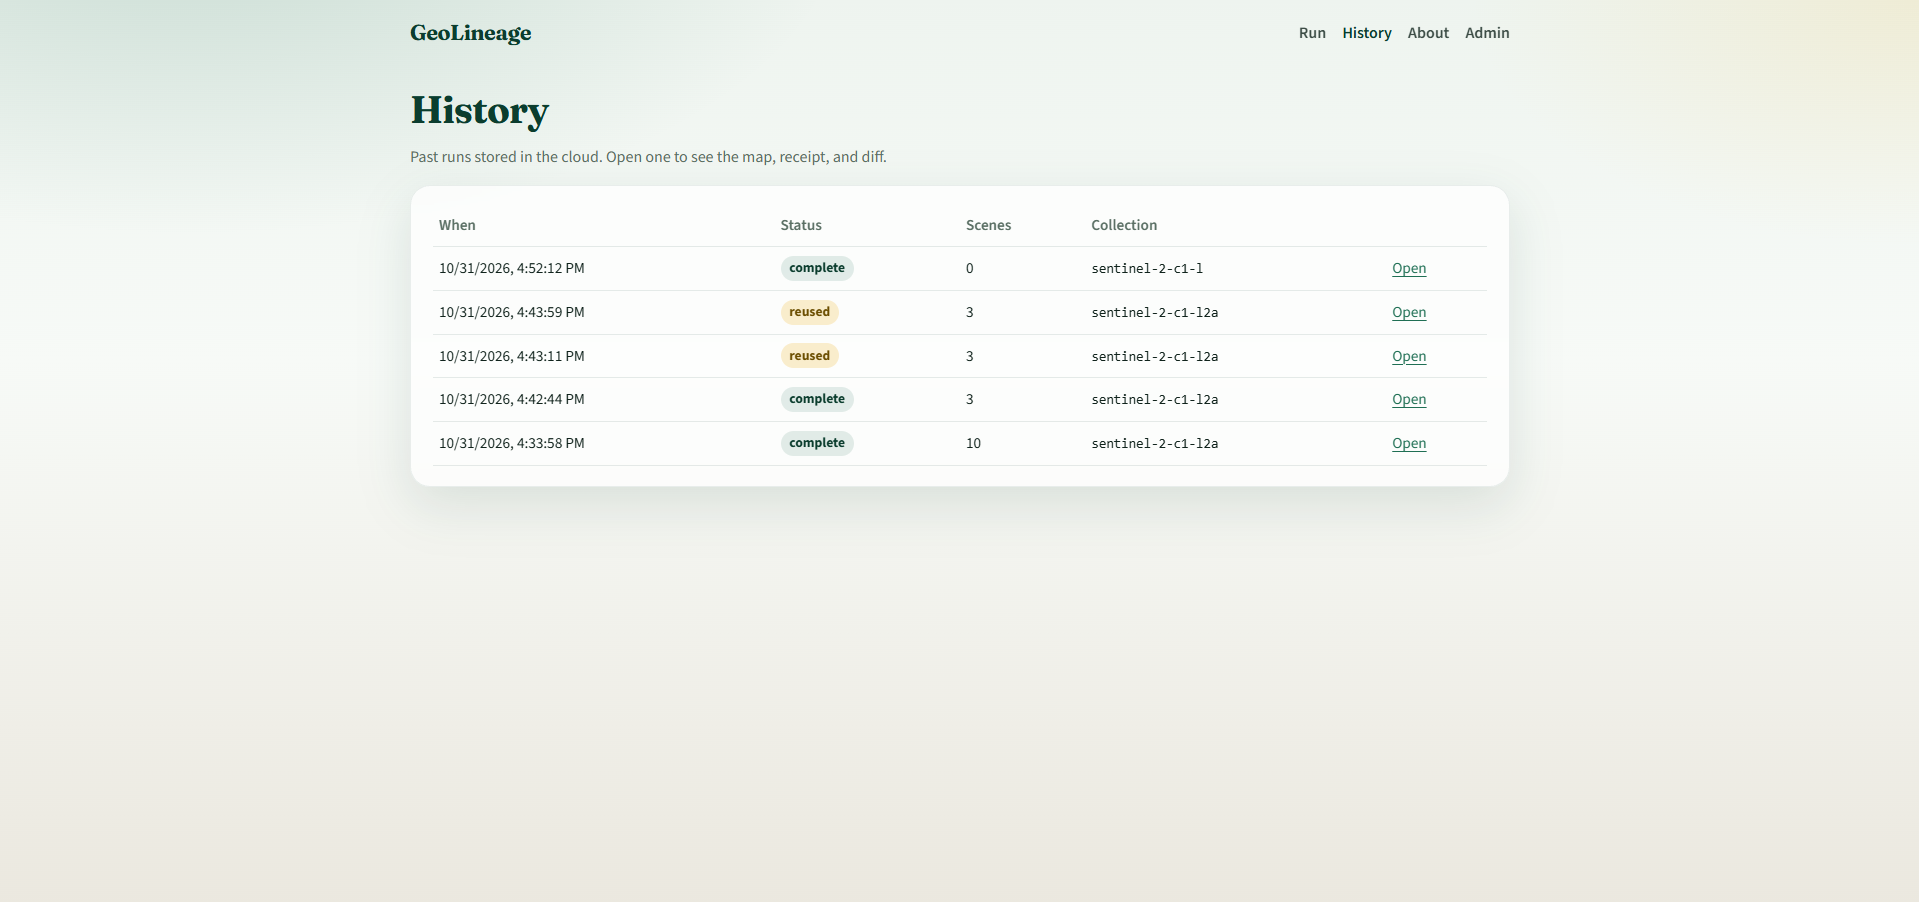
\includegraphics[width=\textwidth]{figures/app_history.png}
\caption{Hosted UI: run history with \texttt{complete} and \texttt{reused} statuses (minimum recompute visible in the audit trail).}
\label{fig:app-history}
\end{figure}

\section{Evaluation}
\label{sec:eval}

\subsection{Metrics and Pass/Fail Criteria}
\begin{itemize}[leftmargin=1.4em]
  \item \textbf{M1 Lineage completeness:} Required fields present; non-empty \texttt{input\_assets}; \texttt{output\_assets} non-empty unless reused; valid UUID; ISO timestamp.
  \item \textbf{M2 Diff partition correctness:} $\mathrm{added}\cup\mathrm{removed}\cup\mathrm{unchanged}=\mathrm{current}\cup\mathrm{previous}$, pairwise disjoint.
  \item \textbf{M3 Reuse behaviour:} When input sets equal, \texttt{reused\_from\_run\_id} set, path/checksum match prior, transform skipped.
  \item \textbf{M4 No duplicate outputs:} Repeated identical runs do not create new product files (filesystem check).
  \item \textbf{M5 Reproducibility rate:} (\#~runs with identical input set leading to reuse) / (total reruns) for fixed parameters.
  \item \textbf{M6 Lineage completeness (query):} For every output, DAG query returns non-empty chain; target 100\% (\texttt{run\_evaluation.py}).
  \item \textbf{M7 Incremental recompute:} Multi-region full vs incremental; time saved $(T_{\mathrm{full}}-T_{\mathrm{inc}})/T_{\mathrm{full}}$ (\texttt{experiment\_incremental\_recompute.py}).
\end{itemize}
\textbf{Decision criteria:} PASS/FAIL as reported by the validation suite and reproducibility script. M5--M7 are reported quantitatively where scripts are run.

\subsection{Baseline Comparison}
With no lineage and naive recompute, three identical runs give three product files and no audit trail. With GeoLineage, the same three runs give one product and three lineage records (Table~\ref{tab:baseline}).

\begin{table}[h]
\centering
\caption{Baseline vs GeoLineage: three identical runs (same bbox, catalog, collection, \texttt{max\_items}).}
\label{tab:baseline}
\small
\begin{tabular}{@{}lccc@{}}
\toprule
\textbf{Approach} & \textbf{\# runs} & \textbf{\# products} & \textbf{\# lineage} \\
\midrule
Baseline (no lineage, naive recompute) & 3 & 3 & 0 \\
GeoLineage & 3 & 1 & 3 \\
\bottomrule
\end{tabular}
\end{table}

\subsection{Experiment A: Same Parameters, Two Runs}
\textbf{Objective.} Verify reuse and consistent lineage when parameters are unchanged and the catalog returns the same items.

\textbf{Setup.} Bbox $(-122.5, 37.5, -122.2, 37.8)$ (San Francisco area), Earth Search, \texttt{sentinel-2-c1-l2a}, \texttt{max\_items}=5. Two consecutive runs.

\textbf{Assumption.} STAC returns deterministic results for the same query over a short interval.

\textbf{Procedure.} Execute the pipeline twice with the same command.

\textbf{Expected behaviour.} First run: new output and lineage; second: reuse message and new lineage pointing at the first path/checksum.

\textbf{Result.} In repeated runs, the second run reuses whenever the catalog returns the same five items. \textbf{Conclusion:} RQ3 demonstrated under the assumption (self-test of Definition~1).

\subsection{Experiment B: Different \texttt{max\_items} (Diff)}
\textbf{Objective.} Verify new output and correct diff when \texttt{max\_items} increases (5$\rightarrow$10).

\textbf{Setup.} Same bbox/catalog as A; first run \texttt{max\_items}=5, second =10.

\textbf{Threat.} Upstream catalog may change between runs; diff reflects query-time results.

\textbf{Expected behaviour.} New product; lineage with 10 inputs; Added~$\geq 1$, Unchanged~$\leq 5$, Removed~$=0$.

\textbf{Result.} Diff shows e.g.\ Added~5, Removed~0, Unchanged~5. \textbf{Conclusion:} RQ2 demonstrated for this parameter change.

\subsection{Experiment C: Cross-Catalog Generality}
\textbf{Objective.} Same pipeline logic and schema across catalogs.

\textbf{Procedure.} One run per catalog (Earth Search; Copernicus) with comparable bbox and \texttt{max\_items}.

\textbf{Result.} Schema-consistent lineage and GeoParquet for both; only \texttt{catalog\_url}, \texttt{collection}, and \texttt{input\_assets} differ---in line with catalog-agnosticism (Contribution~1).

\subsection{Experiment D: Non-Determinism Stress Test}
\textbf{Objective.} Quantify reuse rate, input-set stability, and spurious diff rate under $N$ identical queries (threat: pagination/order~\cite{cannata2025}).

\textbf{Setup.} Same as A; \texttt{max\_items}=5; $N=20$ successive identical runs (\texttt{experiment\_d\_stress.py}).

\textbf{Metrics.} Reuse rate $=(\#\mathrm{reuse})/(N-1)$; input-set stability $=(\#\mathrm{match\ previous})/(N-1)$; spurious diff rate $=(\#\mathrm{added/removed\ with\ unchanged\ user\ params})/(N-1)$.

\textbf{Result.} Reuse $19/19$ (100\%); stability $19/19$ (100\%); spurious diff $0/19$ (0\%) in this window. When catalogs vary, reuse can drop and diff correctly reports change.

\subsection{Automated Validation Suite and Reproducibility Scripts}
\texttt{scripts/validation\_suite.py} runs four PASS/FAIL checks in dedicated dirs: (1)~first run produces output+lineage; (2)~identical second run reuses; (3)~higher \texttt{max\_items} yields new output and proper diff; (4)~required fields and non-empty checksum. Our runs: \textbf{4/4 PASS}. \texttt{reproducibility\_check.py} summarises Experiments~A/B. \texttt{run\_evaluation.py} checks M6 (DAG query completeness; target 100\%). \texttt{experiment\_incremental\_recompute.py} reports M7: e.g.\ three regions, full rebuild $5.52$\,s vs incremental $5.90$\,s with $3/3$ reused (time-saved ratio $-6.9\%$ at this small scale---reuse-check overhead comparable to a fast transform; positive savings expected with heavier transforms). Artifacts land in dedicated directories for third-party verification (Appendix~\ref{app:run}).

\begin{table}[h]
\centering
\caption{GeoLineage features vs requirements.}
\label{tab:features}
\small
\begin{tabular}{@{}p{0.42\textwidth}cc@{}}
\toprule
\textbf{Feature} & \textbf{Yes?} & \textbf{Evidence} \\
\midrule
Lineage emitted every run & Yes & M1 + suite check 4 \\
Diff since previous run & Yes & M2 + Exp.~B \\
Minimum recompute & Yes & M3 + Exp.~A \\
Catalog-agnostic ingestion & Yes & Exp.~C \\
Baseline (fewer output files) & Yes & Table~\ref{tab:baseline} \\
Stress under non-determinism & Yes & M5 + Exp.~D \\
DAG + ``what produced this?'' & Yes & \texttt{query\_lineage.py}, demo \\
Lineage completeness (M6) & Yes & \texttt{run\_evaluation.py} \\
Incremental recompute (M7) & Yes & \texttt{experiment\_incremental\_recompute.py} \\
\bottomrule
\end{tabular}
\end{table}

\section{Discussion}

\subsection{Threats to Validity}
\begin{itemize}[leftmargin=1.4em]
  \item \textbf{External validity:} Results depend on STAC API behaviour (paginate, throttle, reorder). Experiment~D quantifies reuse/stability under repeated identical queries.
  \item \textbf{Construct validity:} $(id,\mathrm{checksum})$ identity is technical, not semantic---especially when catalogs omit checksums.
  \item \textbf{Internal validity:} Transform determinism assumes geometry/datetime fields are present and parsed consistently.
\end{itemize}

\subsection{Limitations}
\label{sec:limitations}
\begin{itemize}[leftmargin=1.4em]
  \item \textbf{Single-step pipeline:} Only footprints$\rightarrow$GeoParquet; no multi-step DAG / step-level recompute.
  \item \textbf{Input identity:} Same id with updated content (new checksum) forces recompute; missing checksums compare by id only.
  \item \textbf{Previous run for diff:} Next-oldest timestamp; pruning the store can change which run is ``previous.''
  \item \textbf{No catalog version pinning:} Query-time state only.
  \item \textbf{Result stability and pagination:} May affect reuse/diff under identical user parameters.
  \item \textbf{Href semantics:} A single href may not uniquely identify multi-asset Items.
  \item \textbf{Lineage schema evolution:} Backward compatibility / migration not implemented.
  \item \textbf{Catalog query semantics:} Default sorting, paging, and \texttt{max\_items} interpretation differ across APIs.
\end{itemize}

\subsection{Future Work}
Align lineage with STAC lineage/DAG proposals and PROV; multi-step DAGs with dependency tracking; non-STAC sources (e.g.\ Overture) with version/release id; raster/derived products (e.g.\ NDVI) with per-step lineage; lineage query API/CLI by \texttt{run\_id}, path, or time range; optional \texttt{SoftwareAgent}/SBOM pins on the receipt; and optional export adapters to PROV/OpenLineage/ISO~19115 demonstrated in companion labs.

\subsection{Implications for GeoAI and Digital Twins}
Knowing which upstream assets and parameters produced a layer matters for GeoAI and digital twins---evaluation, auditing, and rollback. GeoLineage offers a minimal pattern to make STAC inputs and GeoParquet outputs traceable without requiring an external lineage platform for this pipeline class.

\section{Conclusion}
GeoLineage is a minimal, provenance-first GeoETL: every run produces a machine-readable lineage record; ``diff since last run'' reports added, removed, and unchanged inputs; and when the input set is unchanged, the pipeline reuses the previous output (minimum recompute). It is catalog-agnostic and has been run against two STAC sources. Under the conditions tested, the experiments and automated validation suite are \emph{consistent with} the design (they verify the implementation against its own definitions; they are not a comparative evaluation against PROV/OpenLineage/DVC baselines).

\textbf{RQ1} is demonstrated for this pipeline: lineage holds full query parameters and concrete inputs. \textbf{RQ2} is demonstrated by diff correctness under the parameter-change experiments reported here. \textbf{RQ3} is demonstrated by reuse behaviour with an audit trail via \texttt{reused\_from\_run\_id}. We treat these as systems-demo results, not as journal-scale claims of general superiority.

The code is open and runnable as a reference for practitioners and a base for multi-step pipelines or standard lineage formats---aligned with calls for explicit provenance, versioning, and minimal metadata~\cite{cannata2025,nuest2018,nuest2020,closa2019,closa2021,gonzalez2024,thompson2023}. This document is a \textbf{working paper} accompanying an open demo; it is not a peer-reviewed publication.

\paragraph{Code availability.}
Source code ships in two trees that share the same receipt contract: (i)~a thin hosted GeoJSON demo (\texttt{GeoLineageApp/}) and (ii)~the GeoParquet reference CLI plus validation scripts (\texttt{reference-pipeline/}). Experiments reported here (validation suite, reproducibility check, Experiment~D stress test, lineage evaluation, incremental recompute) are grounded in \texttt{reference-pipeline/}; see Appendix~\ref{app:run} and the repository file \texttt{REPRODUCIBILITY.md}.

\appendix
\section{Example Lineage JSON (Minimal)}
\label{app:json}
\begin{lstlisting}
{
  "run_id": "a1b2c3d4-e5f6-7890-abcd-ef1234567890",
  "timestamp": "2026-03-04T12:00:00Z",
  "catalog_url": "https://earth-search.aws.element84.com/v1",
  "search_params": {
    "bbox": [-122.5, 37.5, -122.2, 37.8],
    "collection": "sentinel-2-c1-l2a",
    "datetime": null,
    "max_items": 5
  },
  "input_assets": [
    { "id": "S2A_...", "href": "https://...", "checksum": null }
  ],
  "transform_steps": [
    { "name": "footprints_to_geoparquet", "parameters": { "crs": "EPSG:4326" } }
  ],
  "output_assets": [
    {
      "path": "outputs/<run_id>/footprints.parquet",
      "checksum": "sha256hex...",
      "crs": "EPSG:4326"
    }
  ]
}
\end{lstlisting}

\section{How to Run Validation}
\label{app:run}
From the repository's reference tree (\texttt{reference-pipeline/}), not from the hosted Cloudflare demo:
\begin{lstlisting}[basicstyle=\ttfamily\footnotesize]
cd reference-pipeline
python -m venv .venv
# Windows: .venv\Scripts\pip install -r requirements.txt
# Run validation suite
python -m scripts.validation_suite --bbox -122.5 37.5 -122.2 37.8
python -m scripts.reproducibility_check --bbox -122.5 37.5 -122.2 37.8
python -m scripts.experiment_d_stress --bbox -122.5 37.5 -122.2 37.8 --n 20
python -m scripts.run_evaluation
python -m scripts.experiment_incremental_recompute
\end{lstlisting}
Expected: validation suite prints that all tests PASSED; stress test reports reuse rate, input-set stability, and spurious diff rate; evaluation reports lineage completeness (M6); incremental script reports full vs incremental timings (M7).

\begin{thebibliography}{99}

\bibitem{cannata2025}
Cannata et al. (2025).
The challenges of reproducibility for research based on geodata web services.
\textit{ISPRS Archives}.
\url{https://isprs-archives.copernicus.org/articles/XLVIII-4-W13-2025/87/2025/}

\bibitem{nuest2018}
N\"ust, D., et al. (2018).
Reproducible research and GIScience: an evaluation using AGILE conference papers.
\textit{PeerJ} 6, e5072.
\url{https://peerj.com/articles/5072}

\bibitem{nuest2020}
N\"ust, D., et al. (2020).
Improving reproducibility of geospatial conference papers -- lessons learned from a first implementation of reproducibility reviews.
\textit{Septentrio Conference Series}.
\url{https://septentrio.uit.no/index.php/SCS/article/view/5601}

\bibitem{closa2019}
Closa, G., et al. (2019).
A provenance metadata model integrating ISO geospatial lineage and the OGC WPS.
\textit{Transactions in GIS}.
\url{https://ddd.uab.cat/record/224139}

\bibitem{closa2021}
Closa, G., et al. (2021).
Geospatial queries on data collection using a common provenance model.
\textit{ISPRS International Journal of Geo-Information} 10(3), 139.
\url{https://www.mdpi.com/2220-9964/10/3/139}

\bibitem{zhang2020}
Zhang, W., et al. (2020).
Coupling OGC WPS and W3C PROV for provenance-aware geoprocessing workflows.
\textit{Computers \& Geosciences} 142, 104533.

\bibitem{yue2010}
Yue, P., et al. (2010).
Augmenting geospatial data provenance through metadata tracking in geospatial service chaining.
\textit{Computers \& Geosciences} 36(3), 270--281.

\bibitem{di2013}
Di, L., Shao, Y., and Kang, L. (2013).
Implementation of geospatial data provenance in a web service workflow environment with ISO 19115 and ISO 19115-2 lineage model.
\textit{IEEE TGRS} 51(11), 5112--5122.

\bibitem{ijgi2023}
Provenance in GIServices: A semantic web approach (2023).
\textit{ISPRS IJGI} 12(3), 118.
\url{https://www.mdpi.com/2220-9964/12/3/118}

\bibitem{gonzalez2024}
Gonz\'alez--Cebri\'an, A., et al. (2024).
Standardised versioning of datasets: a FAIR-compliant proposal.
\textit{Scientific Data} 11, 291.

\bibitem{thompson2023}
Thompson, M., et al. (2023).
A proposed FAIR approach for disseminating geospatial information system maps.
\textit{Scientific Data} 10, 582.

\bibitem{howe2022}
Howe, J., and Tullis, J. (2022).
Context for reproducibility and replicability in geospatial unmanned aircraft systems.
\textit{Remote Sensing} 14(17), 4304.

\bibitem{masoclos2017}
Mas\'o, J., Closa, G., et al. (2017).
Fine-grain (feature/attribute) provenance in the geospatial PROV research line.

\bibitem{prov}
W3C. PROV Overview. \url{https://www.w3.org/TR/prov-overview/}

\bibitem{iso19115}
ISO TC 211. ISO 19115 / 19115-2 geographic metadata and lineage.

\bibitem{openlineage}
OpenLineage. Specification / object model. \url{https://openlineage.io/docs/spec/object-model}

\bibitem{stac}
STAC Specification. \url{https://stacspec.org/}

\bibitem{stacproc}
STAC Processing Extension (STAC extensions ecosystem).

\bibitem{geoparquet}
GeoParquet Specification. \url{https://geoparquet.org/}

\bibitem{earthsearch}
Earth Search (Element84) STAC API. \url{https://earth-search.aws.element84.com/v1}

\bibitem{copernicus}
Copernicus Data Space Ecosystem STAC. \url{https://stac.dataspace.copernicus.eu/v1}

\end{thebibliography}

\end{document}
